\begin{center}
\begin{longtable}{ |l|l| } 
 \hline
 Attribute & Description\\ 
 \hline
 timestamp & when the purcahse was made\\ 
 \hline
 txId & ID of the purchase\\ 
 \hline
 userSessionId & ID of the user who made the purchase\\ 
 \hline
 team & is ID of the team that user is in\\ 
 \hline
 userId & is ID of the user that made the purchase\\ 
 \hline
 buyId & ID of purchased item\\ 
 \hline
 price & price of prucased item\\ 
 \hline
\caption{buy-clicks.csv}
\end{longtable}
\end{center}

Dataset buy-clicks appears to not have any missing data.
\begin{figure}[H]
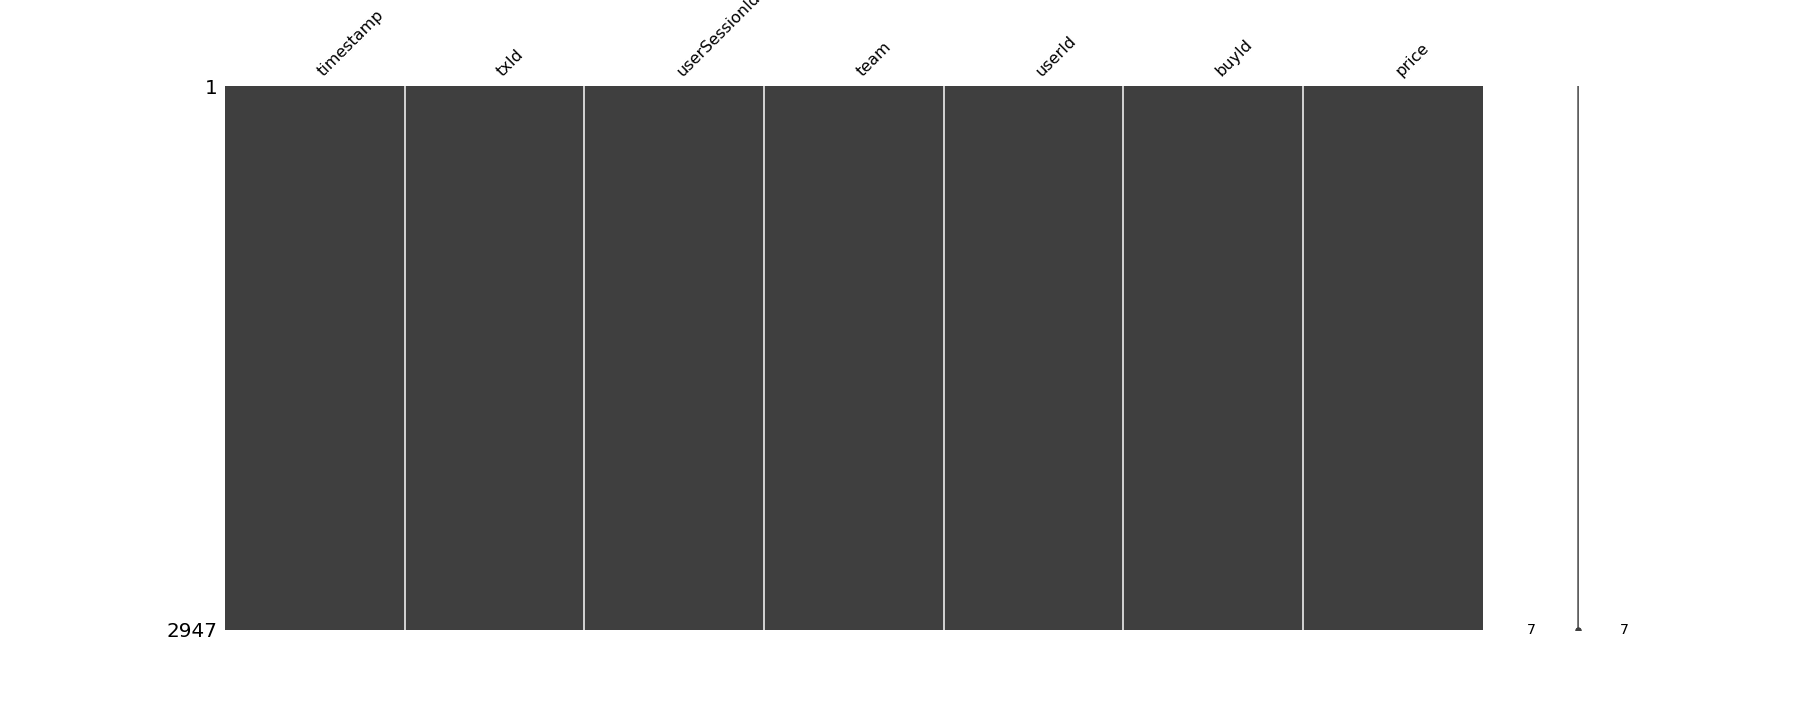
\includegraphics[scale=0.25]{img/Graphs/buyClicks/missingno_buyClicks.png}
\centering
\caption{missingno\_buyClicks}
\label{fig:missingno_buyClicks}
\end{figure}

Looking over the time series, graph is similar to ad-clicks in terms of decline. 
\begin{figure}[H]
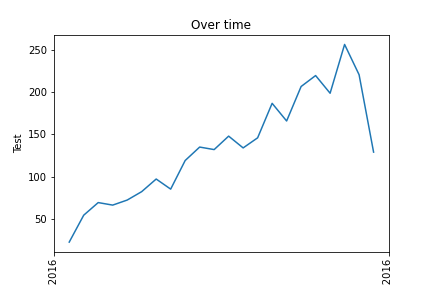
\includegraphics[scale=0.85]{img/Graphs/buyClicks/timeseries_buyClicks.png}
\centering
\caption{timeseries\_buyClicks}
\label{fig:timeseries_buyClicks}
\end{figure}

Investigating which team has bought the most items, we can see that team with id 27 is the top spender although it is only 3rd one in terms of team members. The second biggest spender, team 64, has the most members. This would put team 27 in odd position since they appear to be the perfect team (quite big and they spend the most).
\begin{figure}[H]
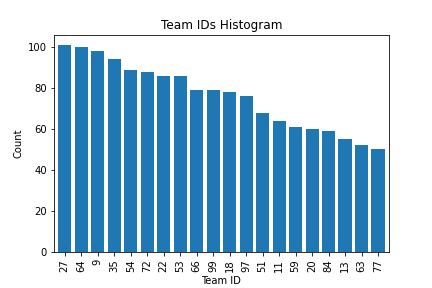
\includegraphics[scale=0.85]{img/Graphs/buyClicks/histogram_buyClicks.png}
\centering
\caption{histogram\_buyClicks}
\label{fig:histogram_buyClicks}
\end{figure}

Creating a correlation chart between team, price and buy ID shows us that team is not correlated to anything. On the other hand, buy id and price seems to be heavily correlated which we have confirmed with missing data in Combined data section (Figure \ref{fig:combinedData_msno}).
\begin{figure}[H]
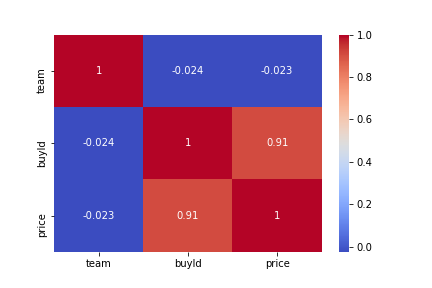
\includegraphics[scale=0.85]{img/Graphs/buyClicks/correlationPlot_buyClicks.png}
\centering
\caption{correlationPlot\_buyClicks}
\label{fig:correlationPlot_buyClicks}
\end{figure}